\documentclass[ansiapaper,12pt]{article}

\usepackage[utf8]{inputenc}

\usepackage[T1]{fontenc}

% \usepackage[ngerman]{babel}

% 215 x 280
\usepackage{geometry}
 \geometry{
 ansiapaper,
 total={160mm,230mm},
 left=25mm,
 top=25mm
 }

\usepackage{helvet}
\renewcommand{\familydefault}{\sfdefault}

\usepackage{hyphenat}
\usepackage{hyperref}

% Load the parskip package without options
% (Without options -> No indent on Paragraph start)
\usepackage{parskip}

\usepackage{graphicx}
\graphicspath{ {./rsc/} }

\begin{document}

\begin{titlepage}
    \begin{center}
        \vspace{2.5cm}

        \Huge
        \textbf{Group Project Proposal}

        \vspace{0.5cm}
        \LARGE
        Human Computer Interaction\\
        COMP 3583

        \vspace{1.5cm}

        \textbf{GeoBlazers}

        \vfill
        \large

        Adam Kremnica - 157683k\\
        Daniel Borwnell - 157827b\\
        Leonard Langer - 0305873l\\
        Patrick Viscount - 154477v\\
        Pulkit Gupta - 161252g

        \vspace{0.8cm}

        \Large
        Date: September 22, 2023\\ %\today\\
        Instructor: Sazia Mahfuz\\

        \vspace{0.5cm}
    \end{center}
\end{titlepage}

\tableofcontents
\newpage

\section{What will the Application do?}
% -> Big Picture goals

Our group decided to create an interactive Acadian map, called GeoBlazers.

We are planning to have it be an interactive map with information on points of interest,
often called a thematic map,
to serve as an interactive virtual tour for new students.

We will use the open street maps api to get a very detailed,
open source map of acadia,
and have the in-game character walk around on the roads and paths across Acadia.

As they get close to any given campus building,
we will have a pop-up for that building that includes the building name,
discipline that studies there,
fun facts and potentially floor plans for each building on campus.

\section{Two similar products and differences}

\subsection{Google Maps}

% \href{http://www.acadiau.ca/~epatters/AMA/campusmap.pdf}{Acadia map}

We are looking to create a fun interactive map that people can use to explore Acadia’s campus.

This is similar to the Acadia Map which is the current standard for our University.

\begin{itemize}
    \item[Difference] We will use vibrant and inviting colours, unlike the current map which is dull and generic.
    \item[Difference] With the current map, you cannot search by building title, instead you have to find the name of the building then match it with its corresponding number on the map (Unintuitive design).
\end{itemize}

\subsection{Mobile Video Game}

\href{http://www.bearbitstudios.com/privacy/}{Smashy Road} is a fixed camera car chase game for mobile devices.

Since it is designed for phones,
the graphics are extremely efficient and easy to understand.

And the fixed camera makes it easy to figure out which car you are controlling.

We would like to mimic this style for our map.

\begin{itemize}
    \item[Difference] Obviously we are not creating a mobile game, we are trying to create a map that students, parents and staff can use.
    \item[Difference] We are creating a map with fixed dimensions versus in Smashy Road the map is procedurally generated.
\end{itemize}

\section{How will we incorporate our classes?}

\subsection{Double Diamond}

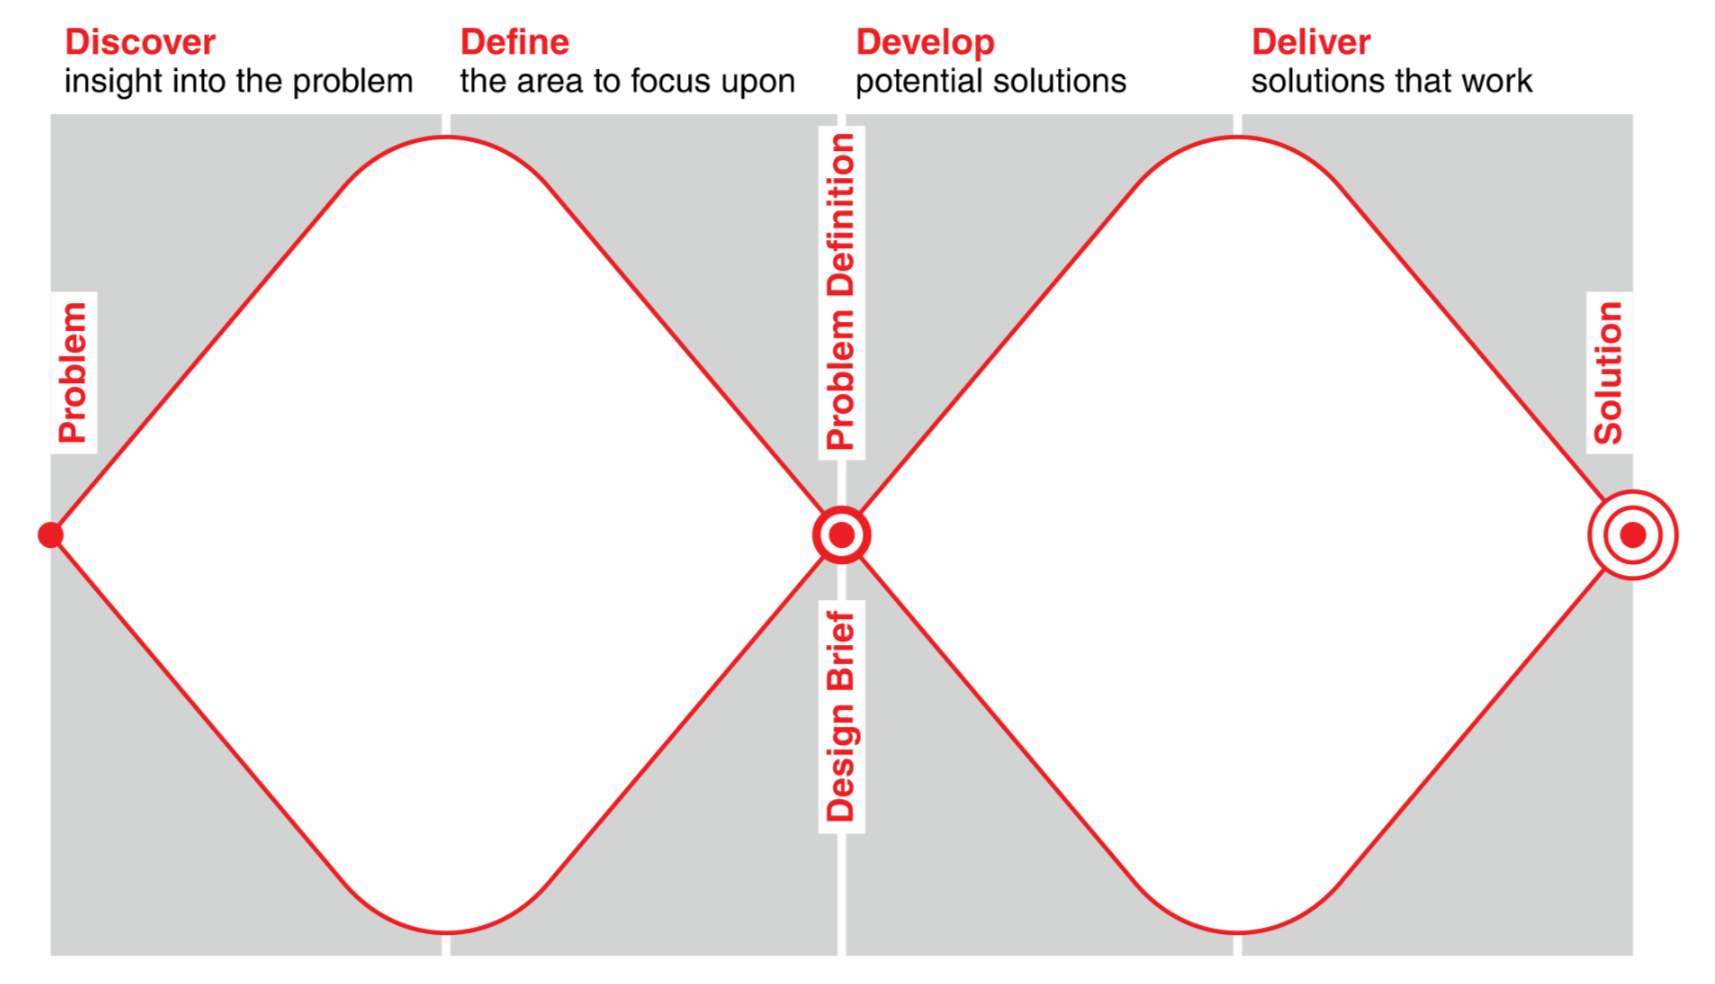
\includegraphics[width=\textwidth]{double-diamond.png}

% Reasons why we are using the Double Diamond model:

\textbf{User-Centered Approach}: The Double Diamond model places a strong emphasis on understanding and empathizing with users. In software development, it's crucial to design solutions that meet the needs and preferences of the end-users. By following the model, software designers are encouraged to gather user insights during the discovery phase, leading to more user-friendly and effective software.

\textbf{Iterative Process}: Software development often requires multiple iterations and refinements. The Double Diamond model inherently supports iteration by allowing designers to revisit and expand upon their ideas at different stages. This iterative approach is well-suited to the evolving nature of software projects.

\textbf{Creativity and Innovation}: The model promotes divergent thinking, which encourages the generation of a wide range of ideas and solutions. In software design, this can lead to innovative features, user interfaces, and functionality.

\textbf{Collaboration}: Software development often involves multidisciplinary teams, including designers, developers, and stakeholders. The Double Diamond model encourages collaboration and cross-functional teamwork. It enables all team members to contribute their expertise and perspectives throughout the design process.

\textbf{Risk Reduction}: By thoroughly exploring and defining the problem space before committing to a solution, the Double Diamond model can help reduce the risk of building software that doesn't meet user needs or has to be extensively reworked later in the development process. This can save time and resources in the long run.

\subsection{User-Centered Design}

Since our product will be used by many people with different backgrounds and experience, we will absolutely need to prioritize our users and involve them in our development.
Some other reasons include:

\textbf{User-Centered Design}: When software is designed with users in mind, it's more likely to fulfill their actual needs and preferences. User feedback ensures that the software aligns with the real-world requirements of its intended audience, making it more relevant and valuable.

\textbf{Issue Identification}: Users often encounter usability issues, bugs, and unexpected behaviors that may not be apparent to the development team. By involving users in testing, you can catch and address these problems early, preventing them from becoming major issues that could delay the software release or lead to user frustration.

\textbf{Validation and Improved UX}: User feedback validates design decisions and helps refine the user experience (UX). This iterative process allows you to make necessary adjustments to the software's interface, features, and functionality, resulting in a more intuitive and user-friendly product. Users who find the software easy to use are more likely to engage with it positively.

\textbf{Competitive Advantage}: Software that incorporates user feedback and testing tends to stand out in the market. It differentiates your product by offering a superior user experience and functionality compared to competitors. Positive user experiences can drive higher user adoption rates and word-of-mouth recommendations.

\subsection{User Accessibility}

Also, ensuring software accessibility is vital because it promotes inclusivity,
expands the potential user base, enhances the user experience, and aligns with legal and ethical obligations.
By making software accessible, organizations embrace inclusivity, meet regulatory requirements,
improve their reputation, and tap into a broader market.

% todo!(“Describe user goals and expectations for wireframe designs”)
% todo!("PM organises google sprints")
% todo!("Took pictures to provide a better UI interface")

\section{What programming language?}

% What?
The project will be implemented in Godot with GDScript, a language similar to
Python3.

% Why?
The reasoning behind this is that it allows us to focus on designing an
optimal user experience, since it alleviates us from implementing a
3d-renderer or collision detection.
Furthermore this decision allows us to quickly iterate on a
user-feedback-based-design without spending much time adapting the
backend.

% Additional Benefits?
The decision to go with a game engine instead of using graphics
frameworks also allows us to build artefacts for different targets
without big changes to the implementation.

% What could be problematic?
Though we also need to be aware of possible shortcomings to this approach.
An immediate problem would be that it is a relatively untested approach to
designing HCI Apps, apart from video games. Another Problem would be that
this project is for an university class and therefore a substantial
part of the code should be the groups own contribution.

% Looking beyond
Depending on how the project evolves the project might use other Languages
apart from Godot/GDScript. An example would be JavaScript to enhance the
exported web version of the App.

\section{Evaluation Method}

Our project team intends on evaluating our app throughout its life cycle inorder to implement the best app possible. To orchestrate this, we intend on using the Double Diamond Design.

\subsection{Double Diamond Design}

Our project team intends on evaluating our app throughout its life cycle inorder to implement the best app possible.
To orchestrate this, we intend on using the Double Diamond Design.

\subsubsection{Discover}

\textbf{Research}: Before we start programming, our focus is on understanding the problem or challenge thoroughly. In this phase, we intend on gathering insights, conducting user research, and empathising with the end-users or stakeholders to gain a deep understanding of their needs and perspectives. For us, that means talking to Acadian students to learn about their Acadia map knowledge, and understand what shortcomings the current solutions may have.

\textbf{Define}: In this phase, our goal is to define and frame the problem based on the insights gained during the research phase. Using the information collected, we will identify key issues, and create a clear problem statement based on that. 

% \subsubsection{Define}
% \dots

\subsubsection{Develop}

\textbf{Ideate}: During this phase we intend on focusing on brainstorming and exploring various solutions to problem statement(s) identified in the last phase. Using sketching and wireframes, we will work as a team to have a cohesive understanding on what we want our app to accomplish moving forward.

\textbf{Prototype}: During this phase, we will create multiple in-depth wireframe designs for an app that has all the parts of the solution that we need based on the previous phase. Then, we will choose a wireframe design (probably a combination of many) to move forward with based on user experience goals from a small subset of testers and the measurable usability goals: 
• Effectiveness • Efficiency • Safety • Utility • Learnability • Memorability

\subsubsection{Deliver}

\textbf{Test}: In this phase, we intend on majorly focusing on developing our app using the designs from the last phase. Our prototypes will then be tested with real users, again measuring the success based on user experience goals and usability goals. We are conducting this testing with the purpose of identifying what works and what doesn't, so we can polish our app in the future. For this testing, we intend on doing A/B testing.
A/B Testing
In development, our team will create two UI menus for our application. Then, using a defined user group, we intend on getting them to use both versions, to tell us the pros and cons of both. Then, using the feedback we receive, we intend on implementing the pros of both into the final application.

\textbf{Implement}: Finally, based on the feedback and insights from testing, the chosen solution is implemented or developed further. This phase majorly involves refining the design, making necessary adjustments based on the results from our A/B Testing.

\section{Breakdown of team roles}

\begin{itemize}
    \item[Adam] Researching potential technologies to incorporate prototypes. Tech stack Identification.
    \item[Daniel] \dots
    \item[Leo] Github (Github Admin) / Researching into CI.
    \item[Patrick] Set meetings and make sure we get there on time
    \item[Pulkit] \dots
\end{itemize}

\end{document}
